
\section{Theorie}
\label{sec:Theorie}

\subsection{Fourier-Analyse}\label{subsec:F-A}
Zeitlich periodische Vorgänge lassen sich durch Funktionen der Form
\[
f(t) = f(t+T)
\]
beschreiben, wobei $T$ die Periodendauer des Vorganges ist.
Nicht zeitlich periodische Vorgänge lassen sich äquivalent beschreiben.
Handelt es sich bei dem betrachteten Vorgang um eine solche zeitlich periodische Funktion, so kann sie nach dem Fourierschen Theorem beschrieben werden durch:
\begin{equation}
f(t) = \frac{\mathrm{a}_.0}{2} + \sum_{n=1}^\infty\left(\mathrm{a}_n\text{ cos}(\omega_nt)+\mathrm{b}_n\text{ sin}(\omega_nt)\right)
\end{equation}
, falls diese Reihe gleichmäßig konvergent ist. 
Dabei stellen die $\omega_n=n\frac{2\pi}{T}=n\omega_.1$ die jeweiligen Kreisfrequenzen der einzelnen Sinus- und Cosinusfunktionen dar. Da $n\in N$ gilt, ist $\omega_.1$ die Grundfrequenz und die $\omega_n$ für $n>1$ sind die harmonischen Oberschwingungen des Systems.
Die Fourier-Koeffizienten $\mathrm{a}_n$ und $\mathrm{b}_n$ lassen sich berechnen nach:
\begin{equation}
\mathrm{a}_n = \frac{2}{T}\int_0^Tf(t)\text{ cos}(\omega_nt)\diff t\text{\hspace{1em}und\hspace{1em}}\mathrm{b}_n=\frac{2}{T}\int_0^Tf(t)\text{ sin}(\omega_nt)\diff t\text{\hspace{1em},}n\in N \label{eq:Koeffizienten}
\end{equation}   
Bei geraden Funktionen verschwinden alle $\mathrm{b}_n$, bei ungeraden alle $\mathrm{a}_n$. 
Trägt man die Fourier-Koeffizienten $\mathrm{a}_n$ und $\mathrm{b}_n$ gegen die Frequenz auf, so erhält man das Spektrum der Schwingung (vergleiche Abbildung \ref{fig:Spektrum}).
\begin{figure}
	\centering
	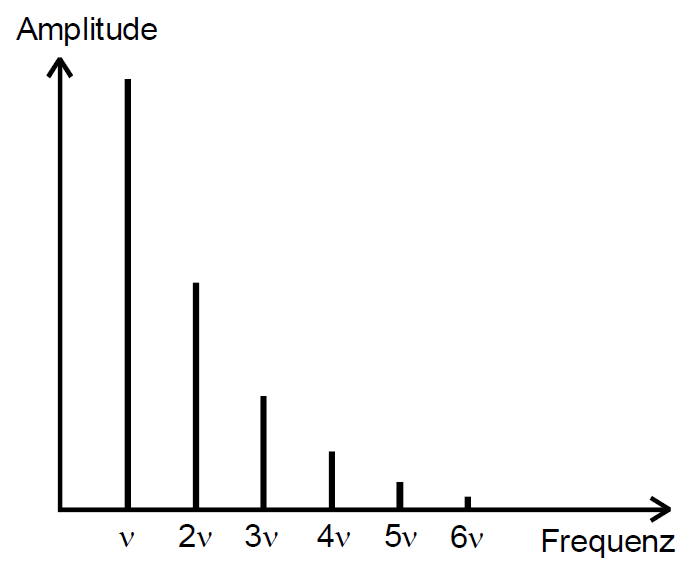
\includegraphics[scale=0.3]{content/images/Spektrum.png}
	\caption{Beispiel für ein Frequenzspektrum\cite{V351}}
	\label{fig:Spektrum}
\end{figure}

\subsection{Fourier-Transformation}\label{F-T}
Mit der oben beschriebenen Fourier-Analyse können nur die Fourier-Komponenten einer periodischen Funktion ermittelt werden. Möchte man das Frequenzspektrum einer beliebigen (hier zeitabhängigen) Funktion $f(t)$ bestimmen, so muss das gesamte Frequenzspektrum $g(\omega)$ der Funktion mittels der Fourier-Transformation bestimmt werden:
\begin{equation}
g(\omega)=\int_{-\infty}^\infty f(t)e^{i\omega t}\diff t\text{.}
\end{equation}  
Bei nicht periodischen Funktionen geht also das Linienspektrum aus \ref{subsec:F-A} in ein kontinuierliches Frequenzspektrum über.\newline
Die Umkehrung der Fourier-Transformation lautet:
\begin{equation}
f(t)=\frac{1}{2\pi}\int_{-\infty}^\infty g(\omega)e^{-i\omega t}\diff\omega\text{.}
\end{equation}  